\documentclass[handout]{beamer}  %%% FÜR HANDOUT ALS PDF

\setbeamertemplate{navigation symbols}{}
\usetheme{Madrid}
\usecolortheme{seagull}
\beamersetuncovermixins{\opaqueness<1>{10}}{\opaqueness<2->{15}}
\usepackage[english]{babel}
\usepackage{csquotes}
\usepackage{graphicx}
\usepackage{verbatim}
\newcounter{saveenumi}
\newcommand{\seti}{\setcounter{saveenumi}{\value{enumi}}}
\newcommand{\conti}{\setcounter{enumi}{\value{saveenumi}}}
\usepackage[hyperref=true,style=authoryear, dashed=false, maxnames=3,backend=bibtex8,doi=false,isbn=false,backref=true]{biblatex}
\usepackage{amssymb,amsmath}
%\setlength{\bibitemsep}{\baselineskip}
\usepackage{xcolor}
\usepackage{graphicx,pstricks,beamerprosper}
\usepackage{subfigure}
\usepackage{verbatim}
\usepackage{cancel}
\renewcommand{\CancelColor}{\red}
\begin{document}
\author[Willi Mutschler]{Willi Mutschler, M.Sc.}
\date{Summer 2013}
\institute[Institute of Econometrics]{Institute of Econometrics and Economic
Statistics\\University of M\"unster\\willi.mutschler@uni-muenster.de}
\title[DSGE methods]{Advanced Macroeconomics (PhD) - DSGE methods}
\subtitle{Estimation methods}

\begin{frame}
\titlepage
\end{frame}

\section{Idea}

\begin{frame}\frametitle{Full information estimation}\framesubtitle{Idea}
    \begin{itemize}
      \item Full information estimation requires a complete characterization of the data-generating-process (not only specific moments).
      \item Consider the linear first-order \emph{state-space} representation of the model:
        \begin{align}
        z_t &= A(\theta) {z}_{t-1} + B(\theta) \varepsilon_{t},  &\text{with }& E[\varepsilon_t]= 0,\quad E[\varepsilon_t \varepsilon_t']=\Sigma_\varepsilon \label{transition}\\
        d_t &= D z_t + \mu_t,& \text{with }& E[\mu_t]=0, \quad E[\mu_t \mu_t']= \Sigma_\mu. \label{observer}
        \end{align}
    \item $z_t=(\widehat{x}_t',\widehat{y}_t')'$ contains all model variables as deviations from steady-state, and $A$ and $B$ are functions of $g_x$ and $h_x$.
    \item Matrix $D$ combines the model variables $z_t$ with observable data variables $d_t$
    \item Equation \eqref{transition}: \emph{state-} or \emph{transition-equation}
    \begin{itemize}
      \item Corresponds to the solution of the model.
      \item $\varepsilon_t$ are the stochastic innovations.
    \end{itemize}
    \item Equation \eqref{observer}: \emph{observation-equation}
    \begin{itemize}
      \item Corresponds to the measurement equations,
      \item subject to possible measurement errors $\mu_t$ in the data.
    \end{itemize}
    \end{itemize}
\end{frame}

\begin{frame}\frametitle{Full information estimation}\framesubtitle{Idea}
  \begin{itemize}
    \item Given distributional assumptions about $\varepsilon_t$ and $\mu_t$, one can derive the log-likelihood-function, $\log{L(d|\theta)}$, analytically or numerically.
    \item In the log-linear case and considering normally distributed variables, the Kalman-filter is used to calculate the likelihood analytically.
    \item In the nonlinear case the policy functions are functions of the vector of parameters $\theta$. The particle-filter or the \emph{efficient importance sampling} is then used to derive the likelihood numerically.
    \item There are two approaches for analyzing and evaluating the log-likelihood:
    \begin{enumerate}
      \item \textbf{the classic (frequentist) \emph{Maximum-Likelihood}-method},
      \item \textbf{the bayesian method}.
    \end{enumerate}
  \end{itemize}
\end{frame}

\section{Kalman-filter}

\subsection{Notation}
\begin{frame}\frametitle{Kalman-filter}\framesubtitle{Notation}
We simplify and consider only the linear case and ignore possible measurement errors in the data:
\begin{itemize}
    \item $d_t = D z_t$
    \item $    z_{t+1} = A z_t + B \varepsilon_{t+1}$
    \item $\varepsilon_{i} \overset{iid}{\sim} \mathcal{N}(0,\Sigma_\varepsilon),~ \Sigma_\varepsilon = E(\varepsilon_{i} \varepsilon_{i}'), ~ E(\varepsilon_{i} \varepsilon_{j}')=0$
  \end{itemize}
\scriptsize
\begin{block}{Notation for the linear projection}
\begin{align*}
{\widehat{z}_{t|t-j}} &= E({z_t}|{d_{t-j}},{d_{t-j-1}},\dots {d_{1}})\\
{\Sigma_{t|t-j}} &= E({z_t}-{\widehat{z}_{t|t-j}})({z_t}-{\widehat{z}_{t|t-j}})'\\
{\widehat{d}_{t|t-j}} &= E({d_t|d_{t-j}},{d_{t-j-1}},\dots,{d_1})\\
{u_t} &= {d_t} - {\widehat{d}_{t|t-1}} = {D} ({z_t} - {\widehat{z}_{t|t-1}})\\
E({u_t}{u_t}')&= {D} {\Sigma_{t|t-1}} {D'}
\end{align*}
for $t=1,2,\dots,T$ and $j=0,1,\dots T$.
\end{block}

\end{frame}

\subsection{Initialization}
\begin{frame}\frametitle{Kalman-filter}\framesubtitle{Initialization}
  \begin{itemize}
    \item Since ${z_t}$ is covariance-stationary, the variance is given by:
\begin{align*}
    \underbrace{E({z_t} {z_t}')}_{\equiv {\Sigma_z}}&=E\left[({A} {z_{t-1}} + {B} {\varepsilon_t})({A} {z_{t-1}} + {B} {\varepsilon_t})'\right] \\
    &= {A} \underbrace{E({z_{t-1}}{z_{t-1}}')}_{\equiv {\Sigma_z}}{A}' + {B} \underbrace{E({\varepsilon_t} {\varepsilon_t}')}_{={\Sigma_\varepsilon}} {B}'\\
\Leftrightarrow {\Sigma_z} &= {A} {\Sigma_z} {A'} + {B} {\Sigma_\varepsilon} {B}'\\
\Leftrightarrow    vec({\Sigma_z}) &= ({I}-{A} \otimes {A})^{-1} vec({B} {\Sigma_\varepsilon} {B}')
\end{align*}
\item \begin{block}{Vectorization}
    The $vec$-operation stacks the rows of a $m\times n$ Matrix ${M}$ into a $mn\times 1$ vector $vec({M})$. Then for arbitrary Matrices $\underset{m\times n}{A}$,$\underset{n\times p}{B}$ and $\underset{p \times k}{C}$:
    \begin{align*}
        vec(ABC) = (C' \otimes A)vec(B), \quad \text{with } \otimes: \text{Kronecker-product.}
    \end{align*}
\end{block}
  \end{itemize}
\end{frame}

\begin{frame}\frametitle{Kalman-filter}\framesubtitle{Initialization}
The unconditional expectation of ${z_1}$ is used for the initialization of the Kalman-filter, since there is no additional information yet:
\begin{align*}
{\widehat{z}_1} &= \underbrace{E({z_1})}_{=E({z})} = {A }\underbrace{E({z_0})}_{=E({z})} + {B}\underbrace{E({\varepsilon_1})}_{=0} \Leftrightarrow {\widehat{z}_1} = {0},\\
vec({\Sigma_{1|0}}) & = E({z_1}-{0})({z_1}-{0})'= vec({\Sigma_z}) = ({I}-{A} \otimes {A})^{-1} vec({B} {\Sigma_\varepsilon} {B}').
\end{align*}

\end{frame}

\subsection{Recursion}
\begin{frame}\frametitle{Kalman-filter}\framesubtitle{Recursion}
The recursion is then given by:
\begin{align*} {\widehat{z}_{t+1|t}} = {A} {\widehat{z}_{t|t}} \end{align*}
\begin{block}{\scriptsize Formula for updating a linear projection (Hamilton (1994,~S.99 und S.379))}
\scriptsize\begin{align*}
  {\widehat{z}_{t|t}} &= {\widehat{z}_{t|t-1}}  +\left[E({z_t}-{\widehat{z}_{t|t-1}})({d_t}-{\widehat{d}_{t|t-1}})'\right] \left[E({d_t}-{\widehat{d}_{t|t-1}})({d_t}-{\widehat{d}_{t|t-1}})'\right]^{-1} {u_t}\\
 \Leftrightarrow {\widehat{z}_{t|t}}&= {\widehat{z}_{t|t-1}}+ {\Sigma_{t|t-1}} {D'} \left({D}{\Sigma_{t|t-1}}{D'}\right)^{-1} {u_t}\\
  \Rightarrow {\widehat{z}_{t+1|t}} = {A} {\widehat{z}_{t|t}} &={A} {\widehat{z}_{t|t-1}}+ {A}{\Sigma_{t|t-1}} {D'} \left({D}{\Sigma_{t|t-1}}{D'}\right)^{-1} {u_t}, \\
  &\qquad\qquad\qquad\qquad\qquad\qquad\qquad~~~ \text{with } {u_t} = {d_t} - {\widehat{d}_{t|t-1}} = ({d_t} - D{\widehat{z}_{t|t-1}}).
\end{align*}
\end{block}
\end{frame}

\begin{frame}\frametitle{Kalman-filter}\framesubtitle{Recursion}
\begin{itemize}
\item ${z_{t+1}} - {\widehat{z}_{t+1|t}} = {A}\left({z_{t}} - {\widehat{z}_{t|t-1}}\right) + {B} {\varepsilon_{t+1}} - {A}{\Sigma_{t|t-1}} {D'} \left({D}{\Sigma_{t|t-1}}{D'}\right)^{-1} {u_t}$
\item The \emph{MSE: } ${\Sigma_{t+1|t} }= E\left({z_{t+1}} - {\widehat{z}_{t+1|t}}\right)\left({z_{t+1}} - {\widehat{z}_{t+1|t}}\right)'$ is given by:
\scriptsize\begin{align*}
    &{\Sigma_{t+1|t} }=\\
    & {A} {\Sigma_{t|t-1}} {A'} + {B} {\Sigma_\varepsilon} {B}' - {A}{\Sigma_{t|t-1}} {D'} \underbrace{\left({D}{\Sigma_{t|t-1}}{D'}\right)^{-1} \underbrace{E({u_t} {u_t'})}_{={D} {\Sigma_{t|t-1}} {D'}}}_{={I}}
    \left({D}{\Sigma_{t|t-1}}{D'}\right)^{-1} {D} {\Sigma_{t|t-1}} {A}'
\end{align*}
\end{itemize}
\scriptsize\begin{block}{Mean-Sqared-Error (MSE)}\centering
$
{\Sigma_{t+1} } \equiv {\Sigma_{t+1|t} }      = {A} {\Sigma_{t|t-1}} {A'} + {B} {\Sigma_\varepsilon} {B}' - {A}{\Sigma_{t|t-1}} {D'} \left({D}{\Sigma_{t|t-1}}{D'}\right)^{-1} {D} {\Sigma_{t|t-1}}{A}'
$
\end{block}
\end{frame}

\subsection{Summary and Likelihood}
\begin{frame}[shrink]\frametitle{Kalman-filter}\framesubtitle{Summary}
The Kalman-filter can be summarized as follows:
\begin{enumerate}
  \item Initialization with
  \begin{itemize}
  \item ${\widehat{z}_1} = {0}$,
  \item $vec({\Sigma_{1|0}}) = ({I}-{A}
      \otimes {A})^{-1} vec({B} {\Sigma_\varepsilon}
      {B}')$.
  \end{itemize}
  \item Period-t likelihood function
  \begin{itemize}
    \item $u_t = ({d_t} - D{\widehat{z}_{t|t-1}})$
    \item $d_{t|t-1} = D \widehat{z}_{t|t-1}$
    \item $\Omega_{t|t-1}:= E(u_t u_t')=D\Sigma_{t|t-1}D$
  \end{itemize}
  \item Period-t filtering density
  \begin{itemize}
    \item ${\widehat{z}_{t|t}}= {\widehat{z}_{t|t-1}}+ {\Sigma_{t|t-1}} {D'} \left({D}{\Sigma_{t|t-1}}{D'}\right)^{-1} {u_t}$
    \item $\Sigma_{t|t}= \Sigma_{t|t-1} - \Sigma_{t|t-1}D' \left({D}{\Sigma_{t|t-1}}{D'}\right)^{-1} D \Sigma_{t|t-1}$
  \end{itemize}
  \item Period-t predictive density
  \begin{itemize}
    \item ${\widehat{z}_{t+1|t}}  ={A} {\widehat{z}_{t|t-1}}+ {A}{\Sigma_{t|t-1}} {D'} \left({D}{\Sigma_{t|t-1}}{D'}\right)^{-1} {u_t}$
    \item ${\Sigma_{t+1}} = {A}
        {\Sigma_{t}} {A'} + {B} {\Sigma_\varepsilon}
        {B}' - {K_t} {D}
        {\Sigma_{t}}{A}'$.
    \end{itemize}
\end{enumerate}
\end{frame}

\begin{frame}\frametitle{Log-Likelihood}
  Given the gaussian assumption about the forecast error ${u_t}$ one can derive the distribution of the data $\underset{n \times 1}{{d_t}}$ conditional on
$({z_t},{d_{t-1}},{d_{t-2}},\dots)$ and set up the log-likelihood function:

\begin{block}{Log-likelihood}
\begin{align*}
\log{ \mathcal{L}({d}|{\theta})} &= \sum_{t=1}^T \log{\mathcal{L}({d_t}|{\theta})}\\ &=-\frac{nT}{2} \log(2\pi) - \frac{1}{2}\sum_{t=1}^{T} \log{|{\Omega_t}|}- \frac{1}{2} \sum_{t=1}^T {u_t}' {\Omega_t}^{-1} {u_t}.
\end{align*}
\end{block}
\end{frame}

\section{Maximum-Likelihood}

\subsection{Idea}
\begin{frame}\frametitle{Maximum-Likelihood}\framesubtitle{Idea}
  \begin{itemize}
    \item \textbf{Approach:} The parameters ${\theta}$ are fixed and the data is a random realization of this specific parametrization.
    \item  The \emph{Maximum-Likelihood}-estimator ${\widehat{\mu}_{ML}}$ is then defined as
    \begin{align*}
    {\widehat{\theta}_{ML}} = \underset{\theta}{\text{argmax}}\left\{ \sum_{t=1}^T \log{\mathcal{L}({d_t}|{\theta})} \right\}.
    \end{align*}
    \item Given some regularity conditions the \emph{ML}-estimator is consistent, asymptotically efficient and asymptotically gaussian.
    \item Uncertainty and inference are based upon the assumptions that \textbf{to each realization of data there corresponds a different vector of parameters that maximizes the likelihood}.
    \item Hint for the estimation of the parameters of a DSGE-model:
    \begin{itemize} \item The dimension of ${d_t}$ must be greater or equal to the dimension of the structural shocks ${\varepsilon_t}$, or otherwise the residual term has a singular variance-covariance-matrix.
    \item If not: Add measurement errors or additional shocks.
  \end{itemize}
  \end{itemize}
\end{frame}




\subsection{Idea}
\begin{frame}\frametitle{Maximum-Likelihood}\framesubtitle{Discussion}
\begin{itemize}
  \item Experience shows that it can be pretty hard and tricky to estimate a DSGE model via Maximum-Likelihood.
  \item Data is often not sufficiently informative, i.e. the likelihood is flat in some directions (identification).
  \item DSGE-models are always misspecified. This can lead to absurd parameter values.
\end{itemize}
\end{frame}
\section{Bayesian methods}
\begin{frame}\frametitle{Bayesian methods}\framesubtitle{Idea}
\begin{itemize}
  \item Based upon the likelihood as well: the complete characterization of the data generating process.
  \item \textbf{Approach:} The parameters ${\theta}$ are random and data ${d}$ is fixed.
  \item The idea is to combine known information (data) with additional believes (\emph{prior-believes}) about the parameters and to get an expression for the conditional probability of the parameters.
  \item Hence, one is able to put more weight on a suspected span of the parameter space.
  \item Bayesian methods are a bridge between calibration and the \emph{Maximum-Likelihood}-method:
\end{itemize}
\textbf{\enquote{Bayesian Inference is a Way of Thinking, Not a Basket of Methods (Christopher Sims)}}
\end{frame}

\begin{frame}\frametitle{Bayesian methods}\framesubtitle{Idea}
  \begin{itemize}
     \item Likelihood-function $\mathcal{L}({d}|{\theta})$ is a conditional density of observed data given the parameters:
$\wp({d}|{\theta})=\mathcal{L}({d}|{\theta})$.
     \item Denote $\wp({\theta})$ as the known prior density of the vector of parameters, then using Bayes-rule:
\begin{align*}
    \wp({\theta}|{d}) = \frac{\mathcal{L}({d}|{\theta})\wp({\theta})}{\wp({d})} =  \frac{\mathcal{L}({d}|{\theta})\wp({\theta})}{\int \wp({\theta}) \mathcal{L}({d|{\theta}}) ~d{\theta}} \propto \mathcal{L}({d}|{\theta})\wp({\theta}),
\end{align*}
with $\propto$ meaning \enquote{proportional to}.

     \item $\wp({d})$ is the \emph{marginal likelihood} of the data and ultimately only a constant that normalizes the expression to unity. It is independent of the parameters.
    \item Removing it doesn't change the form of the posterior density $\wp({\theta}|{d})$, it merely doesn't integrate to one.
     \item This non-normalized density is called \emph{posterior-kernel} or, in logs, \emph{log-posterior-kernel}.
   \end{itemize}
\end{frame}

\begin{frame}\frametitle{Bayesian methods}\framesubtitle{Idea}
  \begin{itemize}
    \item The mode is the Bayesian estimator ${\widehat{\theta}_B}$ of the true parameter vector:
\begin{align*}
    {\widehat{\theta}_B} = \underset{\theta}{\text{argmax}}\left\{\log{\wp({\theta}|{d})}\right\} = \underset{\theta}{\text{argmax}}\left\{ \log{\mathcal{L}({d}|{\theta})} + \log{\wp({\theta})} \right\}
\end{align*}
    \item Procedure: Calculate the log-likelihood with the Kalman-filter and simulate the \emph{log-posterior-kernel} through \emph{sampling-} or \emph{Monte-Carlo}-methods.
    \item  In the literature -- and in Dynare -- the \emph{Metropolis-Hastings-algorithm} is commonly used.
    \item  Inference can then be conducted via the properties of the posterior-distribution.
  \end{itemize}
\end{frame}

\subsection{Metropolis-Hastings-algorithm}
\begin{frame}\frametitle{Bayesian methods}\framesubtitle{Metropolis-Hastings-algorithm}
\begin{block}{An and Schorfheide (2007, S.~132)}
  The algorithm constructs a Gaussian approximation around the posterior mode and
  uses a scaled version of the asymptotic covariance matrix as the covariance
  matrix for the proposal distribution. This allows for an efficient
  exploration of the posterior distribution at least in the neighborhood of
  the mode.
\end{block}
\begin{itemize}
  \item The algorithm uses the fact that under very general regularity conditions the moments of a distribution are asymptotically normal.
\item It constructs a sequence of draws (Markov-chains) from a proposal density.
\item This does not need to be identical with the posterior density. It is only required that the algorithm can draw samples from the whole range of the posterior density.
\end{itemize}
\end{frame}


\begin{frame}\frametitle{Bayesian methods}\framesubtitle{Metropolis-Hastings-algorithm}
\begin{itemize}
  \item The current candidate (draw) ${\theta^*}$ is dependent on the previous candidate ${\theta^{(s-1)}}$.
  \item Weights for all candidates are the same, however, they are only accepted with a certain probability $\alpha$, calculated as the ratio of the \emph{posterior-kernel} of the current to the one of the previous candidate.
  \item Due to this construct the algorithm tends to shift the draws from areas of low posterior probability to areas of high probability.
  \begin{itemize}
    \item If ${\theta^{(s-1)}}$ is in an area of high posterior probability, it is likely that only candidates in the same area are accepted.
    \item If ${\theta^{(s-1)}}$ is in an area of low posterior probability, it is very likely that new candidates are accepted.
  \end{itemize}
\item The covariance-matrix of the proposal distribution plays a major role, since it is important to set $\alpha$ neither too large nor to small.
\item Current practice uses the covariance matrix of the mode ${\widehat{\theta}_B}$ and scales it with a factor $c$ such that the average acceptance probability is between 20\% and 30\%.
\end{itemize}

\end{frame}

\begin{frame}\frametitle{Bayesian methods}\framesubtitle{Metropolis-Hastings-algorithm}
\begin{enumerate}
\item Specify $c_0,c$ and $S$.
  \item Maximize $\log{\mathcal{L}({d}|{\theta})} +
      \log{\wp({\theta})}$ using numerical methods.\\
      ${\widehat{\theta}_B}$ denotes the mode.
  \item Calculate the inverse of the Hessian evaluated at the mode, denote it with ${\Sigma_B}$.
  \item Specify an initial value ${\theta^{(0)}}$ or draw it from
      $\mathcal{N}({\widehat{\theta}_B},c_0^2{\Sigma_B})$.
\seti
\end{enumerate}

\end{frame}


\begin{frame}\frametitle{Bayesian methods}\framesubtitle{Metropolis-Hastings-algorithm}
\begin{enumerate}\conti
  \item For ${s}=1,\dots,S$:
  \begin{itemize}
    \item Draw ${\theta^*}$ from the candidate-generating distribution (proposal density)
        $\mathcal{N}({\mu^{(s-1)}},c^2{\Sigma_B})$.
    \item Calculate the acceptance probability $\alpha$:
        \begin{align*}
        \alpha \equiv \alpha\left({\theta^{(s-1)}},{\theta^*}\right) = \frac{\mathcal{L}\left({\theta^{*}}|{d}\right)~\wp\left({\theta^*}\right)}{\mathcal{L}\left({\theta^{(s-1)}}|{d}\right)~\wp\left({\theta^{(s-1)}}\right)}
        \end{align*}
    \item With probability
        $\text{min}\left\{\alpha,1\right\}$ accept the jump from ${\theta^{(s-1)}}$ to ${\theta^*}$.
        In other words: If $\alpha\geq1$, set ${\theta^{(s)}}={\theta^*}$.
    \item With complementary probability don't accept the jump, i.e. draw a uniformly distributed random variable $r$ between $0$ and $1$:
        \begin{itemize}
        \item If $r\leq\alpha$ set ${\theta^{(s)}}={\theta^*}$ (jump).
        \item If $r>\alpha$ set ${\theta^{(s)}}={\theta^{(s-1)}}$ (don't jump).
         \end{itemize}
  \end{itemize}
\seti
\end{enumerate}

\end{frame}

\begin{frame}\frametitle{Bayesian methods}\framesubtitle{Metropolis-Hastings-algorithm}
\begin{enumerate}\conti
  \item Estimate the posterior expectation of a function
      $\hbar({\theta})$ with $\frac{1}{S}\sum_{s=1}^S
      \hbar\left({\theta^{(s)}}\right)$.
  \item If the average acceptance probability does not yield a desirable value (typically between $20\%-30\%$) or the algorithm does not converge, change $c_0,c$ or $S$.
\end{enumerate}

\end{frame}

\subsection{Remarks}
\begin{frame}\frametitle{Bayesian methods}\framesubtitle{Remarks}
  \begin{itemize}
    \item Bayesian estimation of a DSGE-model requires that the number of shocks is equivalent to the numbers of observable variables.
    \item Common choice for priors: gaussian, (normal, shifted or inverse) Gamma, Beta or the uniform distribution.
    \item Choosing a proper prior one has to consider lower and upper bounds as well as the skewness and kurtosis of the distribution.
    \item The results can vary due to the choice of priors and their parametrization.
    \item Therefore one has to check the robustness of the results:
    \begin{itemize}
      \item Try a different parametrization.
      \item Try more general priors.
      \item Noninformative priors.
      \item Sensitivity analysis.
    \end{itemize}
  \end{itemize}
\end{frame}


\subsection{Inference, forecast, model comparison and identification}

\begin{frame}\frametitle{Properties of the Posterior-distribution}
\begin{itemize}
  \item The posterior density combines all information about ${\theta}$: information after the data is observed as well as information prior to the data.
  \item Bayesian estimation works for every sample size, however, it has also the following asymptotic properties:
    \begin{enumerate}
      \item The priors become irrelevant for the determination of the posterior.
      \item The posterior converges to a degenerate distribution around the true value.
      \item The posterior is approximately gaussian.
    \end{enumerate}
  \item Using the posterior distribution one can
  \begin{itemize}
  \item set up Bayesian confidence intervals (credibility sets),
  \item calculate forecasts using the predictive-density: $\mathcal{L}({d_f}|{d})= \int \mathcal{L}({d_f}|({\theta}|{d})){d} {\theta} = \int \mathcal{L}({d_f}|{\theta},{d})\wp({\theta}|{d}){d}{\theta}$
  \item compare models.
\end{itemize}
\end{itemize}
\end{frame}

\begin{frame}\frametitle{Model comparison}
  \begin{itemize}
    \item Models can differ in their prior distribution, the likelihood and the parameters.
    \item Bayesian approach: Calculate the probability that model $i$ is the true model, given the data.
    \item Suppose there are $i=1,2$ models $M_i$ with prior probability $p_i=P(M_i)$ that model $M_i$ is the true model.
    \item Each model has a set of parameters ${\theta_i}$ with a prior distribution $\wp_i({\theta_i})$ and a likelihood $\mathcal{L}_i({d}|{\theta})$.
    \item Then the probability of model 1 being the true model given the data, is given by:
    \scriptsize\begin{align*}
      P(M_1|d) &= \frac{P(M_1)\mathcal{L}_1({d}|M_1)}{\mathcal{L}({d})} = \frac{p_1 \int \mathcal{L}_1({d},{{\theta_1}}|M_1)d {\theta_1}}{\mathcal{L}({d})}\\
      &= \frac{p_1 \int \mathcal{L}_1({d}|{\theta_1},M_1) \wp_1({\theta_1}|M_1) d {\theta_1}}{\mathcal{L}({d})}\\
      \text{with }& \mathcal{L}({d}) = p_1 \int \mathcal{L}_1({d}|{\theta_1},M_1)\wp_1({\theta_1}|M_1)d{\theta_1} + p_2 \int \mathcal{L}_2({d}|{\theta_2},M_2)\wp_2({\theta_2}|M_2)d{\theta_2}
    \end{align*}
  \end{itemize}
\end{frame}

\begin{frame}\frametitle{Model comparison}
  \begin{itemize}
      \item The expected value of the likelihood given the prior distribution is the so-called \emph{marginal-likelihood} for model i:
    \begin{align*}
      m_i({d}) = \int \mathcal{L}_i({d}|{\theta_i},M_i)\wp_i({\theta_i}|M_i)d{\theta_i}
    \end{align*}
    \item Using this, one can calculate the \emph{posterior-odds}:
    \begin{align*}
      PO_{12} = \frac{P(M_1|{d})}{P(M_2|{d})} = \underbrace{\frac{p_1}{p_2}}_{\text{Prior-Odds-Ratio}}\cdot \underbrace{\frac{m_1({d})}{m_2({d})}}_{Bayes-factor}
    \end{align*}
    \item Together with $P(M_1|{d}) + P(M_2|{d}) =1$ one gets the \emph{posterior-model-probabilities}:
    \begin{align*}
      P(M_1|{d}) = \frac{PO_{12}}{1+PO_{12}}, \qquad P(M_2|{d}) = 1-P(M_1|{d}).
    \end{align*}
  \end{itemize}
\end{frame}

\begin{frame}\frametitle{Model comparison}
  \begin{itemize}
    \item The \emph{marginal likelihood} measures the quality of a model to characterize data.
    \item The \emph{Posterior-Odds} don't hint to the true model. They solely describe which model, compared to the other, has the highest conditional probability.
    \item A $PO_{12}>>1$ is an indication that the data as well as the priors prefer model 1.
    \item Guidelines of Jeffrey (1961):
    \begin{itemize}
      \item $1:1 - 3:1\quad~~$ weak evidence for model 1,
      \item $10:1 - 100:1~$ strong evidence for model 1,
      \item $> 100:1\qquad~~$ decisive evidence for model 1.
    \end{itemize}
    \item Implementation and calculation of the integrals is done by numerical MCMC- and sampling-methods, as well as Laplace- or Harmonic-Mean-approximation.
  \end{itemize}
\end{frame}


\begin{frame}\frametitle{Identification}
  \begin{block}{General problem} For a mathematical expression with many conditions and parameters, but only a limited sample, there can exist different combinations of parameters that yield the same result and a similar dataset.\end{block}
  \begin{itemize}
    \item Consider two vectors of parameters ${\theta_1}$ and ${\theta_2}$ for which
    \begin{align*}
    \mathcal{L}({d}|{\theta_1}) = \mathcal{L}({d}|{\theta_2}).
    \end{align*}
    \item If ${\theta_1} = {\theta_2}$, then there is identification. If, however, ${\theta_1} \neq {\theta_2}$, then one does not know which vector of parameters has generated the data.
  \end{itemize}
\end{frame}

\begin{frame}\frametitle{Identification}
\begin{itemize}[<+->]
  \item Simple example: Consider the following ARMA(1,1)-process
  \begin{align*}
  x_t = \phi_1 x_{t-1} + \varepsilon_t -\phi_2 \varepsilon_{t-1}, \text{ with } \varepsilon \sim N(0,\sigma^2)
\end{align*}
with parameter vector $\theta=(\phi_1,\phi_2,\sigma)'$:\pause
\begin{figure}[htbp]
  \subfigure[$\theta_0=(0.4,0.4,1)'$]{
    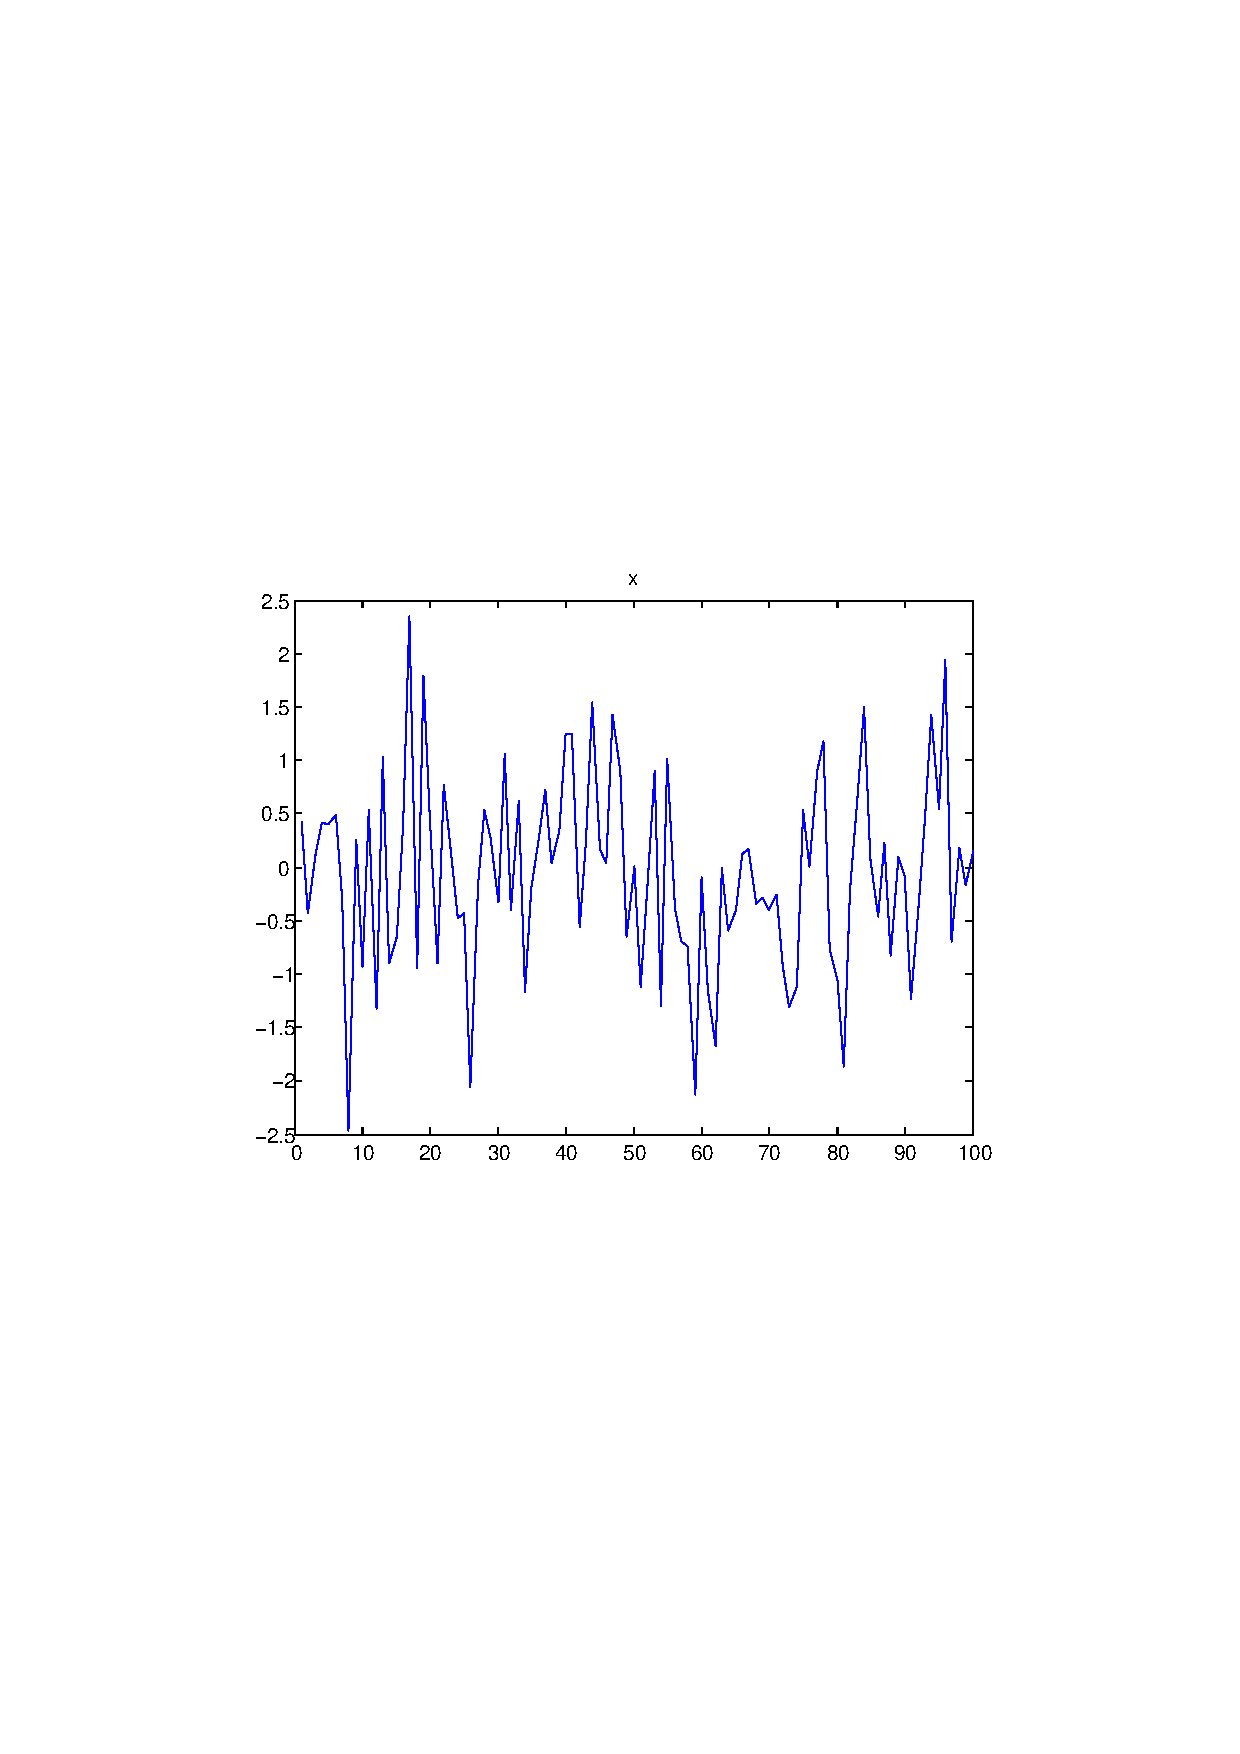
\includegraphics[width=0.35\textwidth]{Grafiken/ARMA1.pdf}
  }
  \subfigure[$\theta_1=(0,0,1)'$]{
    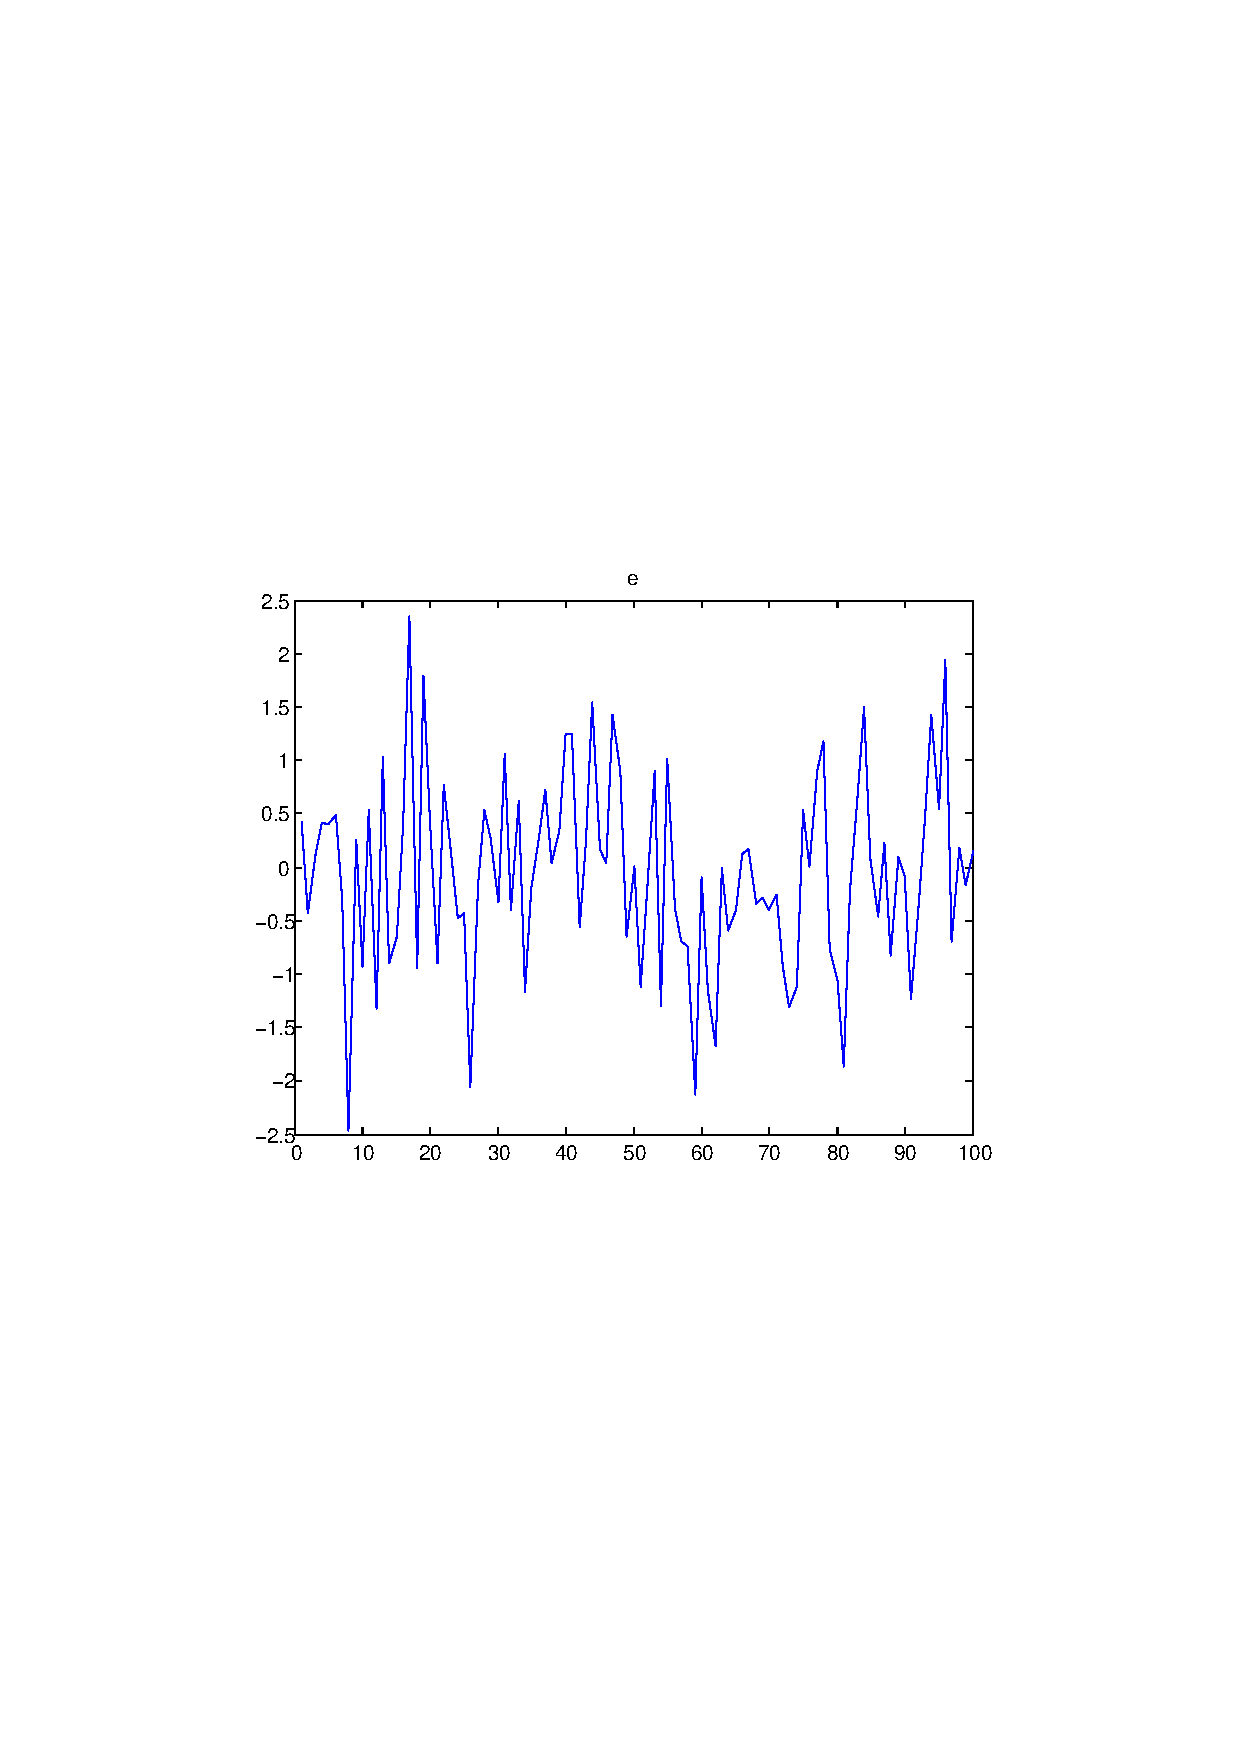
\includegraphics[width=0.35\textwidth]{Grafiken/ARMA2.pdf}
  }
\end{figure}
\item Obviously both models generate the same data (as long as the shocks $\varepsilon_t$ are the same). $\theta_0$ and $\theta_1$ are observationally equivalent.
\item Note $\sigma=1$ is \textbf{partially identifiable}.
\end{itemize}
\end{frame}


\begin{frame}\frametitle{Identification}
\begin{itemize}
  \item Identification is a mathematical problem (dependencies).
  \item Identification problems arise if distinct parameter values do not lead to distinct probability distributions of the data.
  \item Drawing inferences from the probability distribution leads thus to wrong conclusions from estimation and inference.
  \item When identification fails, properties of estimators change.
  \item Even with an infinite sample it is not possible to pin down some parameters, no matter what estimation procedure one uses.
  \item Identification can be studied prior to estimation.  
  \item Identification tests: Order and rank conditions, via autocovariances, spectral densities, information matrix, imposing restrictions, Bayesian methods \dots
\end{itemize}
\end{frame}


\section{Discussion}

\begin{frame}\frametitle{Discussion of full information estimators}
  \begin{itemize}
       \item More restrictive assumptions are needed compared to the limited information estimation: specification of the distribution of the schocks, i.e. the likelihood.
    \item Advantages of a \emph{Maximum-Likelihood}-estimation lie in the full characterization of the data-generating-process and the exact, consistent and efficient estimation of the parameters.
    \item \enquote{Dilemma of absurd parameter estimates}: Problem of the ML-estimation due to wrong distributional assumptions, problems in the optimization algorithm or non-separable identifiable parameters.
    \item Even transformations, upper and lower bounds, etc. are only limited to help overcome this problem, when the likelihood is flat.
  \end{itemize}


\end{frame}

\begin{frame}\frametitle{Discussion of full information estimators}
  \begin{itemize}
    \item This is where Bayesian methods come in and bridge the gap between calibration and the \emph{ML-principle}.
    \item Considering priors one can incorporate additional information into a model.
    \item \enquote{Dilemma of absurd parameter estimates}: Even with Bayesian means it is not possible to estimate these parameters (the posterior looks almost the same as the prior), but one can assign probability such that these parameters are very unlikely.
    \item[$\Rightarrow$] Using priors one can exclude these absurd parameter estimates.
    \item Nevertheless the point of robustness and identification of the parameters remains a critical topic.
  \end{itemize}
\end{frame}

\begin{frame}\frametitle{Discussion of full information estimators}

\begin{block}{An und Schorfheide (2006, S.124)}
Once one acknowledges that the DSGE model provides merely an approximation to
the law of motion of the time series (\dots), then it seems reasonable to
assume that there need not exist a single parameter vector (\dots), that
delivers, say, the \enquote{true} intertemporal substitution elasticity or
price adjustment costs and, simultaneously, the most precise impulse
responses to a technology or monetary policy shock. Each estimation method is
associated with a particular measure of discrepancy between the
\enquote{true} law of motion and the class of approximating models.
\end{block}
\end{frame}

\subsection{Exercise 5: Estimation with Bayesian methods}

\begin{frame}\frametitle{Exercise: Estimation with Bayesian methods}
Consider the following simplified RBC-model (social planer problem);
\begin{align*}
  \underset{\{c_{t+j},l_{t+j},k_{t+j}\}_{j=0}^\infty}{max} W_t &= \sum_{j=0}^\infty \beta^j u(c_{t+j},l_{t+j})\\
  s.t.\quad y_t &= c_t + i_t, & A_t &= A e^{a_t}, \\
  y_t &= A_t f(k_{t-1},l_t), & a_t &= \rho a_{t-1} + \varepsilon_t,\\
  k_t &= i_t +(1-\delta)k_{t-1}, &  \varepsilon_t &\sim N(0,\sigma_{\varepsilon}^2),
\end{align*}
where preferences and technology follow:
\begin{align*}
  u(c_t,l_t)= \frac{\left[c_t^\theta (1-l_t)^{1-\theta}\right]^{1-\tau}}{1-\tau}, \qquad f(k_{t-1},l_t)=\left[\alpha k_{t-1}^\psi + (1-\alpha)l_t^\psi\right]^{1/\psi}.
\end{align*}
Optimality is given by:
\begin{eqnarray*}
 &u_c(c_t,l_t) - \beta E_t \left\{u_c(c_{t+1},l_{t+1}) \left[A_{t+1} f_k(k_t, l_{t+1})+1-\delta \right]\right\} = 0,\\
 & -\frac{u_l(c_t,l_t)}{u_c(c_t,l_t)}-A_t f_l(k_{t-1},l_t)=0,\\
 & c_t + k_t -A_t f(k_{t-1},l_t) -(1-\delta)k_{t-1}=0.
\end{eqnarray*}
\end{frame}

\begin{frame}\frametitle{Exercise: Estimation with Bayesian methods}
\begin{enumerate}[(a)]
  \item Write a mod-file for this model (with a sensible calibration and a steady-state block).
  \item Simulate a sample of 10000 observations for $c_t,l_t$ and $y_t$ using \texttt{stoch\_simul} and save it in a mat-file.
  \item Define priors for $\alpha,\theta$ and $\tau$ (or a different set of parameters).
  \item Estimate the posterior mode using the \texttt{estimation} command and a limited sample with 100 observations. How man observable variables do you need? Check the posterior mode using \texttt{mode\_check}. If you get errors due to a non-positive definite Hessian, try a different optimization algorithm or change the initial values.
\seti
\end{enumerate}
\end{frame}

\begin{frame}\frametitle{Exercise: Estimation with Bayesian methods}
  \begin{enumerate}[(a)]\conti
      \item If you are satisfied with the posterior mode, approximate the posterior distribution using the the Metropolis- Hastings-Algorithmus with $3\times 5000$ iterations. If it does not converge to the (ergodic) posterior-distribution, repeat the algorithm without discarding the previous draws.
  \item How robust are the results regarding the specification of the priors? Repeat the estimation of the posterior-mode for different priors.
\seti\end{enumerate}
\end{frame}
\end{document}
